% !TeX root = ../../main.tex
\section{Model implementation on COMSOL or gPROMS}
%subpoints tbc
\subsection{Model equations}
\subsubsection{1-D model}
\subsubsection{2-D model}




\subsection{Final results}
See \cref{fig:comsol-performance}.

\begin{figure}[h]
    \centering

    \begin{subfigure}{0.49\linewidth}
        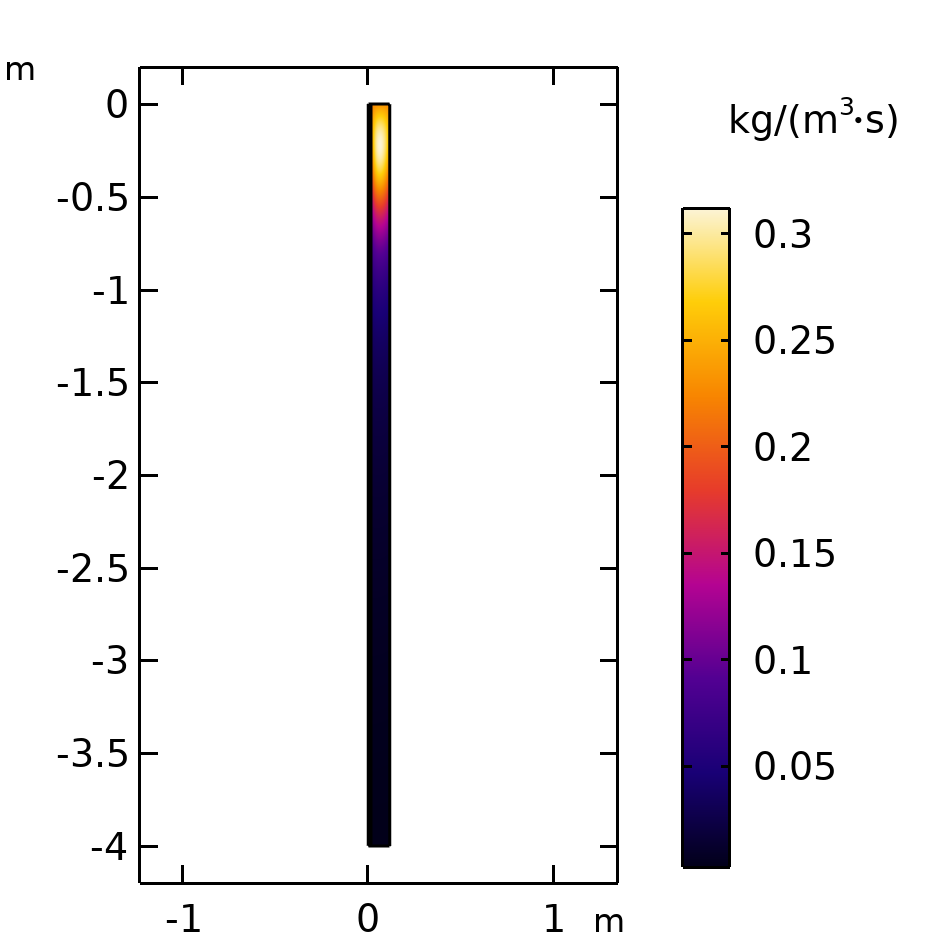
\includegraphics[width=\linewidth]{figures/r_TOL.png}
        \caption{Rate of Toluene reaction}
        \label{fig:comsol-performance:r_TOL}
    \end{subfigure}
    \begin{subfigure}{0.49\linewidth}
        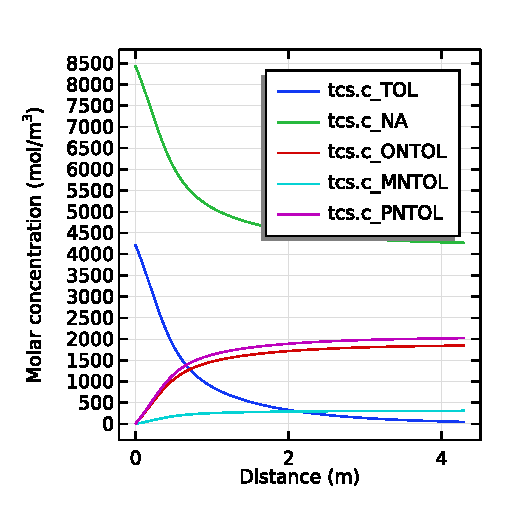
\includegraphics[width=\linewidth]{figures/concentration.eps}
        \caption{Concentration profile within reactor}
        \label{fig:comsol-performance:concentration}
    \end{subfigure}

    \caption{Reactor performance}
    \label{fig:comsol-performance}
\end{figure}

\subsubsection{Conversion}

See \cref{fig:comsol-conversion}.

\begin{figure}[h]
    \centering

    \begin{subfigure}{0.49\linewidth}
        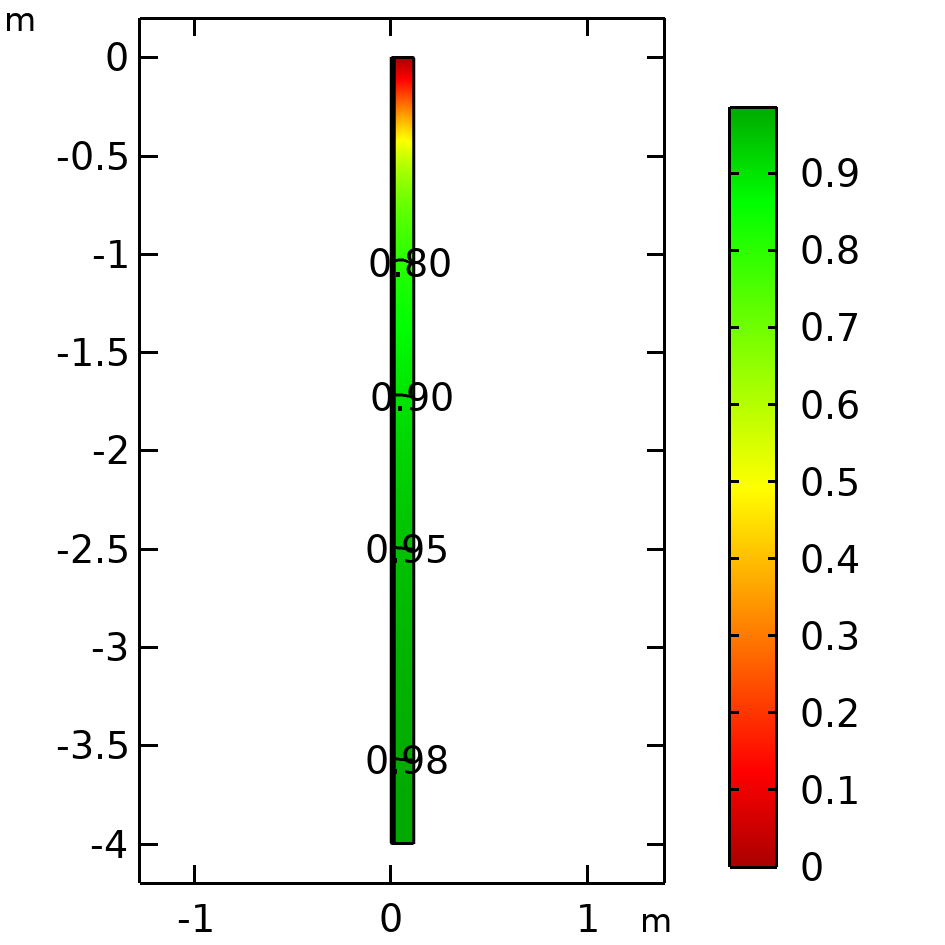
\includegraphics[width=\linewidth]{figures/conversion-surface.png}
        \caption{}
        \label{fig:comsol-conversion:surface}
    \end{subfigure}
    \begin{subfigure}{0.49\linewidth}
        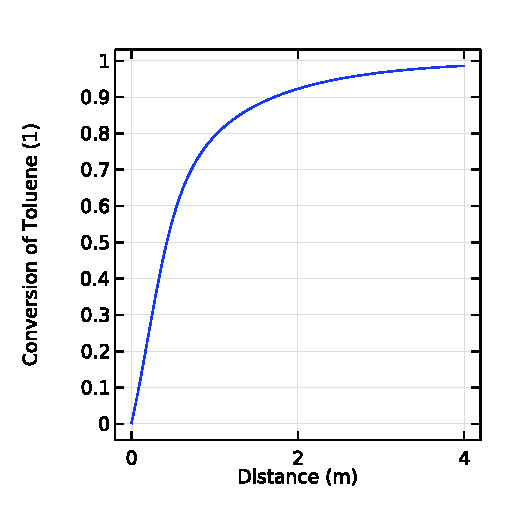
\includegraphics[width=\linewidth]{figures/conversion-line.eps}
        \caption{}
        \label{fig:comsol-conversion:line}
    \end{subfigure}

    \caption{Conversions}
    \label{fig:comsol-conversion}
\end{figure}

\subsubsection{Temperature}

See \cref{fig:comsol-temperature}.

\begin{figure}[h]
    \centering

    \begin{subfigure}{0.49\linewidth}
        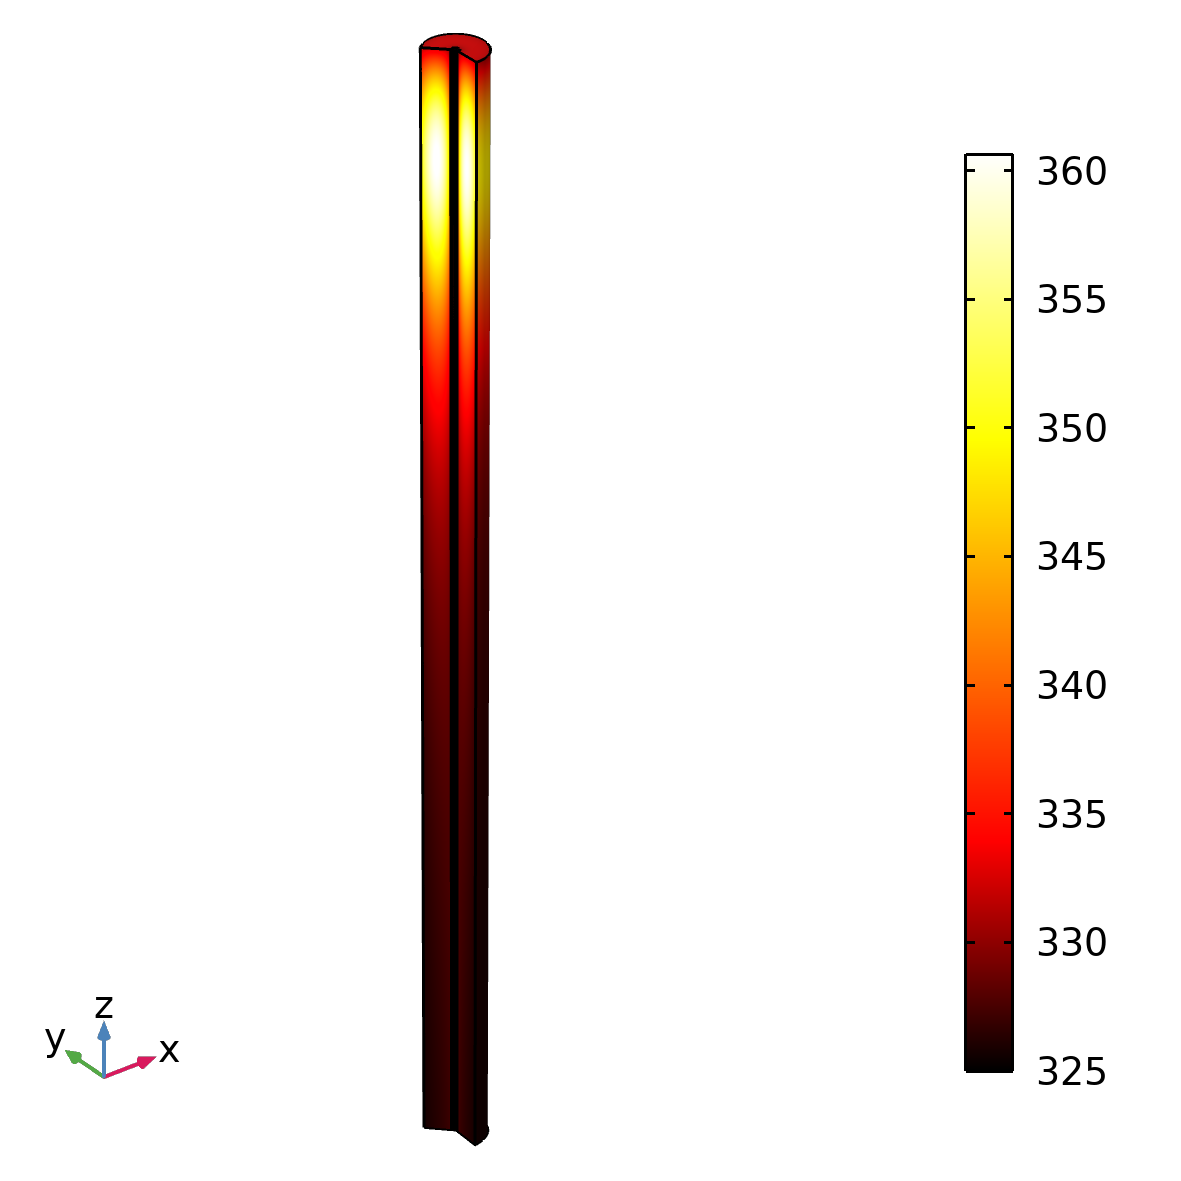
\includegraphics[width=\linewidth]{figures/temperature-surface.png}
        \caption{}
        \label{fig:comsol-temperature:surface}
    \end{subfigure}
    \begin{subfigure}{0.49\linewidth}
        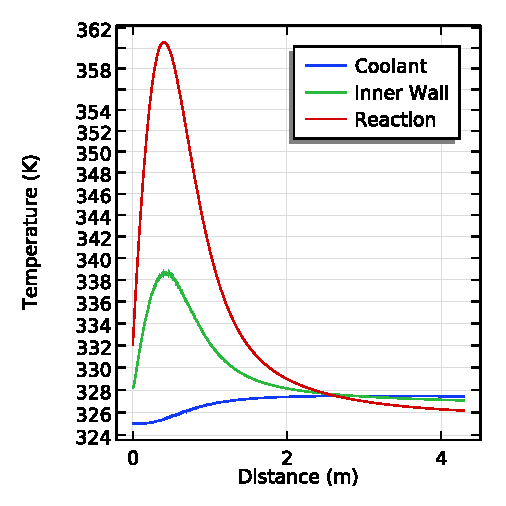
\includegraphics[width=\linewidth]{figures/temperature-lines.eps}
        \caption{}
        \label{fig:comsol-temperature:lines}
    \end{subfigure}

    \caption{Temperatures}
    \label{fig:comsol-temperature}
\end{figure}

\subsection{Optimisation and sens}

\subsubsection{Secondary cooling system sizing}

\begin{figure}[h]
    \centering

    \begin{subfigure}{0.49\linewidth}
        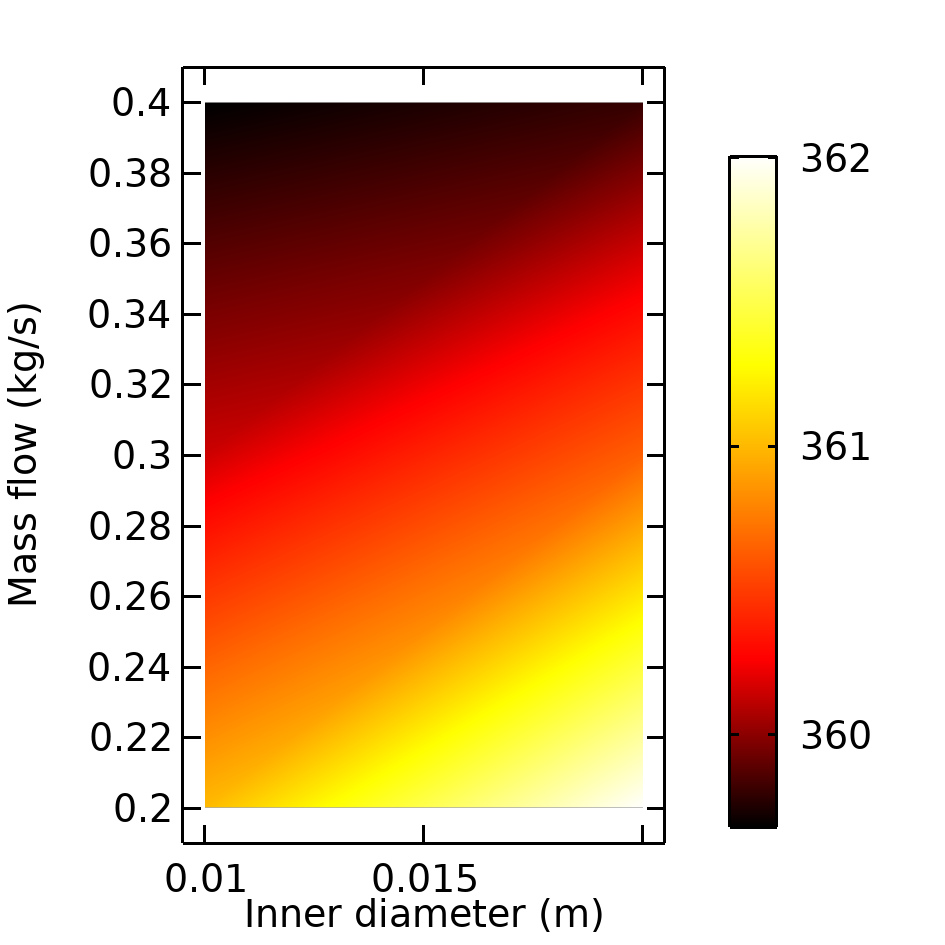
\includegraphics[width=\linewidth]{figures/S2-maxT.png}
        \caption{Maximum temperature reached in the reactor}
        \label{fig:comsol-S2:maxT}
    \end{subfigure}
    \begin{subfigure}{0.49\linewidth}
        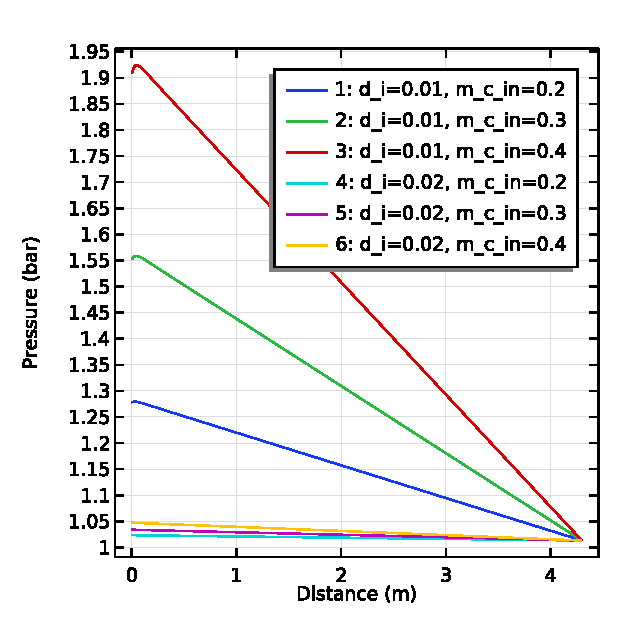
\includegraphics[width=\linewidth]{figures/S2-CW-Pdrop.eps}
        \caption{CW side pressure drop}
        \label{fig:comsol-S2:CW-Pdrop}
    \end{subfigure}

    \caption{Sensitivity to secondary CW parameters}
    \label{fig:comsol-S2}
\end{figure}

\subsubsection{Cocurrent vs counter-current cooling water flow}

\subsubsection{Toluene: \ch{HNO3} ratio}

\subsubsection{Number of tubes}

\subsubsection{Pareto frontier}
MATLAB \texttt{gamultiobj}

\subsubsection{Coolant temperature}
Extra length to allow for variations in T

\begin{figure}[h]
    \centering
    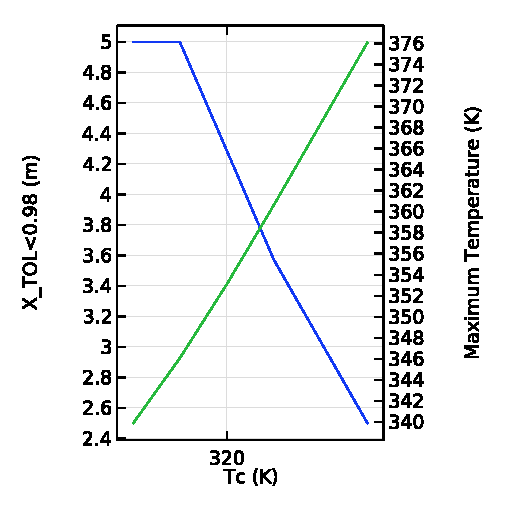
\includegraphics[width=0.49\linewidth]{figures/S4-CW-X-T.eps}
    \caption{Effect of CW temp on conversion and max T}
    \label{fig:comsol-S4-CW-X-T}
\end{figure}
